\documentclass[10pt]{article}
\usepackage[margin=0.75in]{geometry}
\usepackage{graphicx,booktabs,array}
\usepackage[T1]{fontenc}
\usepackage[hidelinks]{hyperref}
\title{Watermark comparisons: paper assets}
\author{}
\date{19 September 2026}
\begin{document}
\maketitle
\noindent All results are completion-only at nominal $p<.001$. See REPORT.md for complete protocols, caveats, numerical paths, provenance, and unfavorable results. No matched empirical FPR claim is made. The paired studies use 50 prompts with two responses each; the historical comparison uses 500 responses per setting.
\begin{figure}[p]
\centering
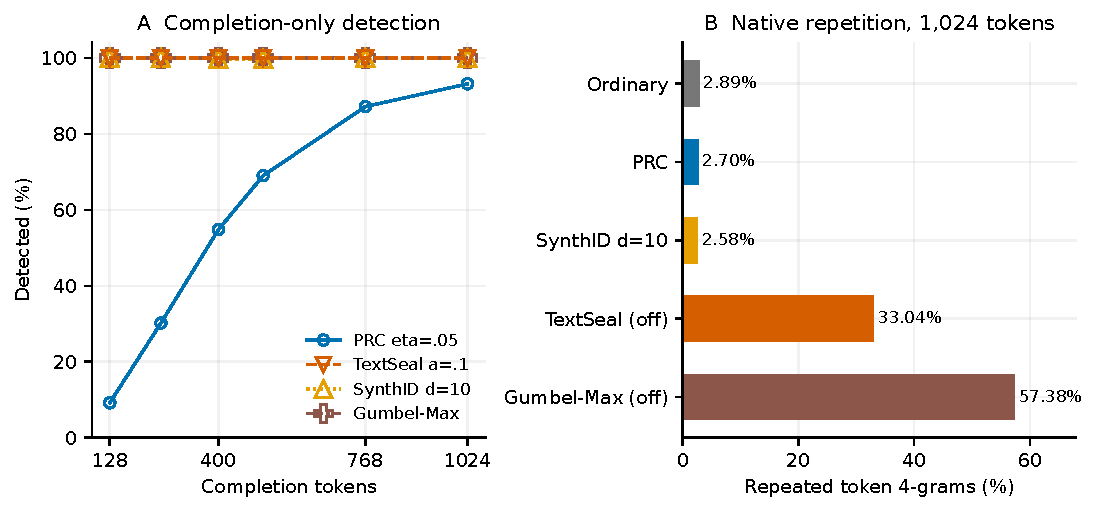
\includegraphics[width=\textwidth]{figures/01_redetection.pdf}
\caption{Historical 500-response-per-setting comparison after completion-only correction. Left: each cutoff is a separate one-shot detection test; coincident baseline curves are retained. Right: 1,024-token repetition under the native mixed policies, with TextSeal/Gumbel fallback OFF. These repetition gaps are not the matched-policy result.}
\label{fig:01_redetection}
\end{figure}
\begin{figure}[p]
\centering
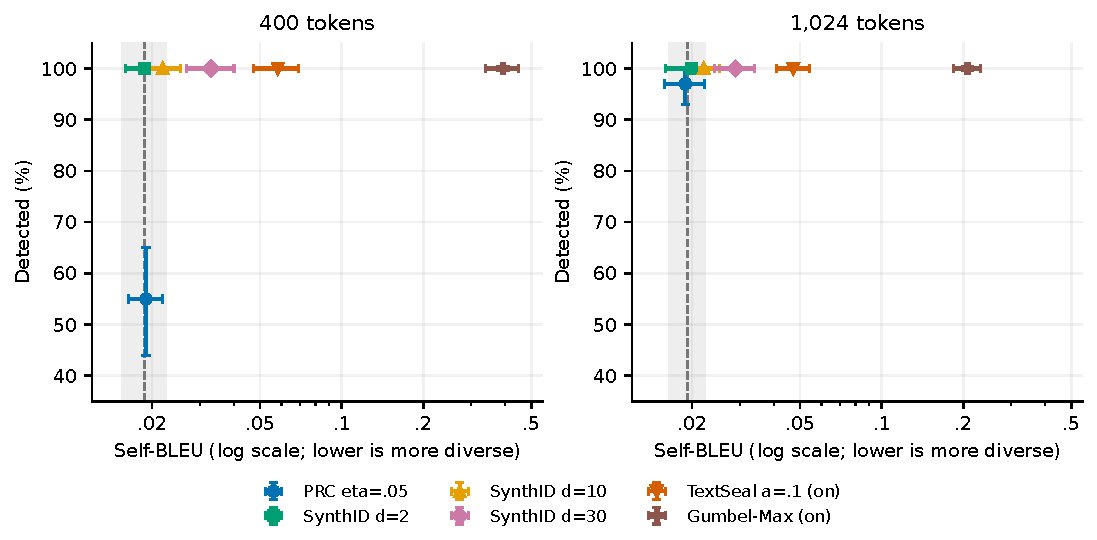
\includegraphics[width=\textwidth]{figures/02_matched_policy_tradeoff.pdf}
\caption{8B T=1 comparison with fallback ON for all contextual baselines, at 400 and 1,024 tokens. Points and error bars show means and marginal 95\% prompt-bootstrap intervals. Ordinary Self-BLEU is a gray vertical mean/band because ordinary text has no watermarked TPR. The logarithmic Self-BLEU axis retains Gumbel without hiding the near-ordinary settings. This is a set of tested configurations, not a fitted frontier or equal-FPR comparison.}
\label{fig:02_matched_policy_tradeoff}
\end{figure}
\begin{figure}[p]
\centering
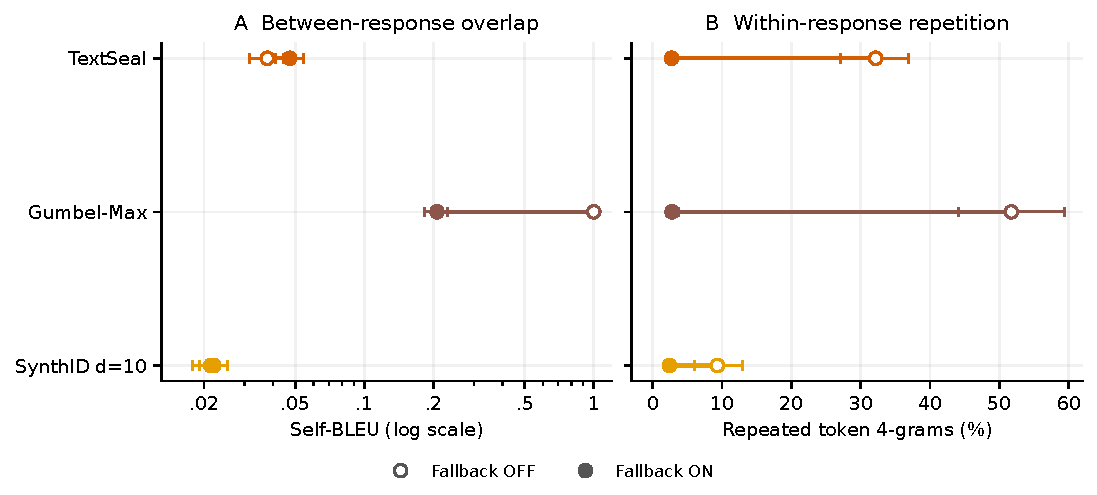
\includegraphics[width=\textwidth]{figures/04_repeat_policy.pdf}
\caption{Repeat fallback at 1,024 tokens: open circles are OFF, filled circles ON; each line connects the same method under the two policies. Left: between-response Self-BLEU on a log scale. Right: within-response repeated-four-gram fraction. Marginal 95\% intervals are shown; paired policy effects are reported in the tables. Reduced within-response repetition need not reduce between-response overlap.}
\label{fig:04_repeat_policy}
\end{figure}
\begin{figure}[p]
\centering
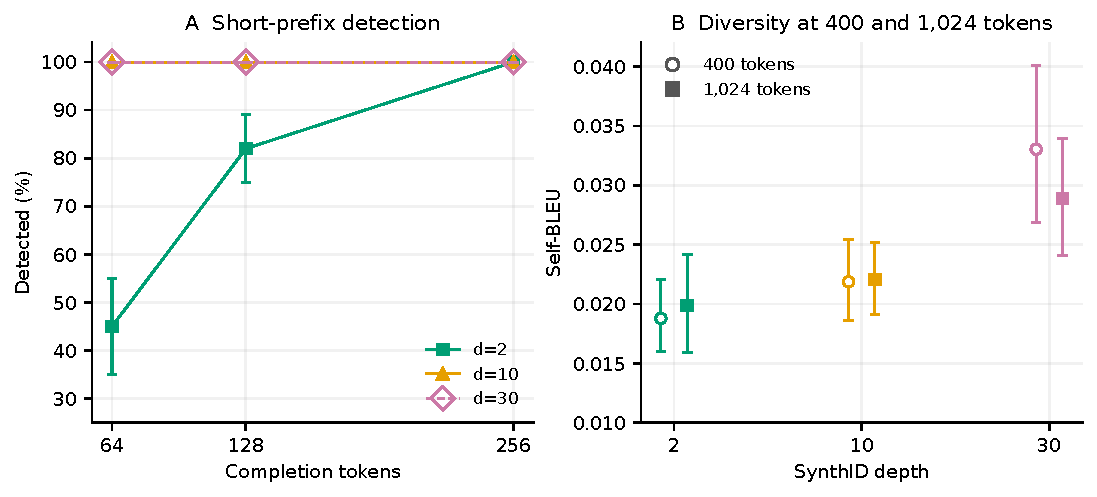
\includegraphics[width=\textwidth]{figures/05_synthid_depth.pdf}
\caption{SynthID depth comparison on saved 8B full-vocabulary T=1 responses. Left: detection at 64/128/256 tokens with prompt-bootstrap intervals; depth-10 and depth-30 curves coincide. Right: Self-BLEU at the original 400/1,024-token endpoints. Depth 30 adds observed overlap without an observed detection gain over depth 10 on these measured cutoffs; no population equivalence or Bayesian-detector claim follows.}
\label{fig:05_synthid_depth}
\end{figure}
\begin{figure}[p]
\centering
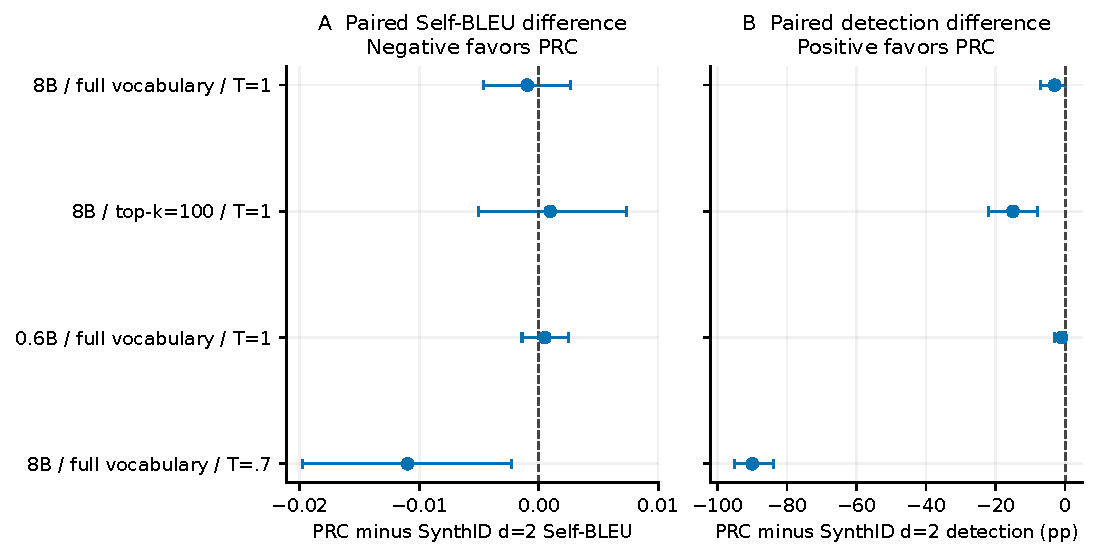
\includegraphics[width=\textwidth]{figures/03_paired_depth2.pdf}
\caption{Direct paired PRC-minus-SynthID-depth-2 contrasts at 1,024 tokens. Left: Self-BLEU differences, where negative favors PRC. Right: detection differences in percentage points, where positive favors PRC. Error bars are paired prompt-bootstrap 95\% intervals. Rows are separate matched-control experiments, not a pure one-factor model-size/truncation sweep; probability arithmetic differs for top-100 and 0.6B. The T=.7 study preserves the original 8B paths.}
\label{fig:03_paired_depth2}
\end{figure}
\begin{figure}[p]
\centering
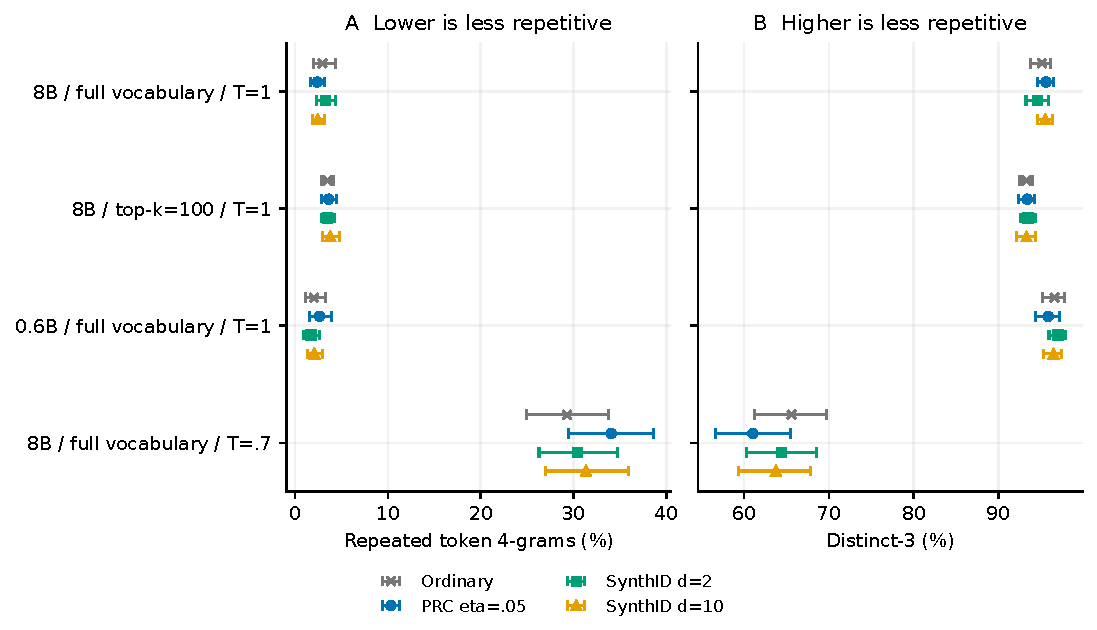
\includegraphics[width=\textwidth]{figures/06_repetition_sensitivity.pdf}
\caption{Within-response repetition at 1,024 tokens across the four completed regimes, showing ordinary, PRC, and SynthID depths 2/10. Error bars are marginal 95\% prompt-bootstrap intervals. Cross-regime numerical paths differ as documented. These metrics concern individual responses and should not be substituted for between-response Self-BLEU.}
\label{fig:06_repetition_sensitivity}
\end{figure}
\begin{figure}[p]
\centering
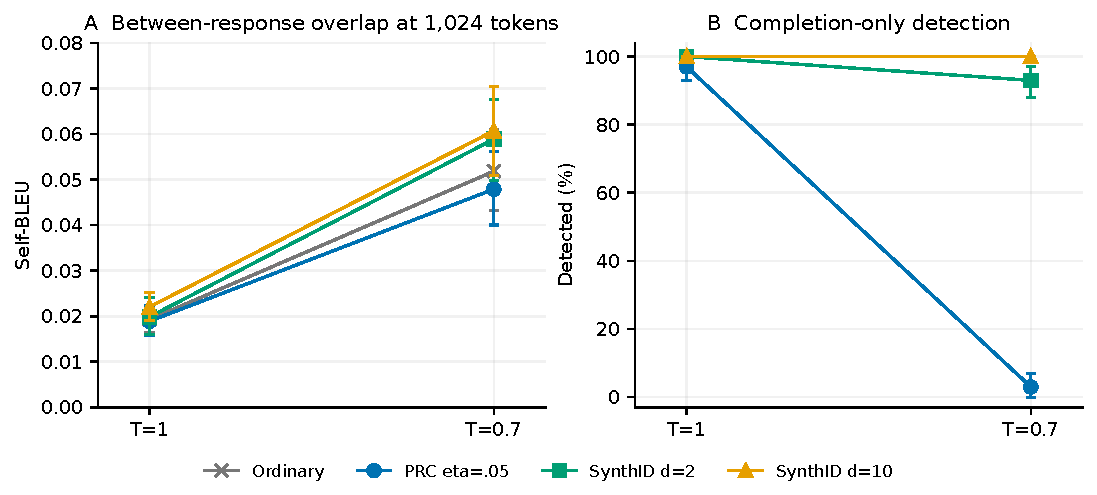
\includegraphics[width=\textwidth]{figures/08_temperature.pdf}
\caption{The precision-faithful 8B full-vocabulary temperature sensitivity at 1,024 tokens. T=1 uses saved original outputs; T=.7 uses new matched controls. Left: Self-BLEU rises for every arm at the lower temperature. Right: PRC detection falls from 97/100 to 3/100, depth 2 from 100/100 to 93/100, and depth 10 remains 100/100. Intervals use prompt resampling; lines connect the two evaluated temperatures and do not imply an unmeasured sweep.}
\label{fig:08_temperature}
\end{figure}
\begin{figure}[p]
\centering
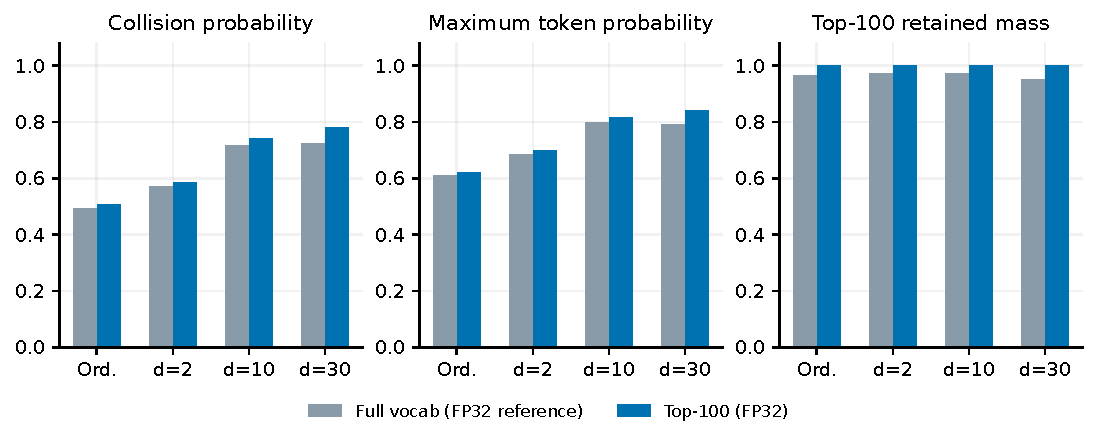
\includegraphics[width=\textwidth]{figures/07_common_histories.pdf}
\caption{Means on 25 preselected shared histories. Collision probability is the sum of squared token probabilities; maximum probability is the largest token probability. Retained mass is on the ordinary top-100 support after watermarking. Both decoders use FP32 arithmetic, so this controlled distribution probe is distinct from reproducing the historical BF16 full-vocabulary pipeline. No causal claim about whole-response Self-BLEU is inferred from these descriptive means.}
\label{fig:07_common_histories}
\end{figure}
\clearpage
% Generated from hash-pinned saved results. Requires booktabs, graphicx and array.
\begin{table*}[t]
\centering
\caption{Completed experiments and their non-overlapping roles}
\label{tab:01_experiment_ledger}
\small
\resizebox{\textwidth}{!}{%
\begin{tabular}{>{\raggedright\arraybackslash}p{\dimexpr0.250000\textwidth-2\tabcolsep\relax}>{\raggedright\arraybackslash}p{\dimexpr0.250000\textwidth-2\tabcolsep\relax}>{\raggedright\arraybackslash}p{\dimexpr0.250000\textwidth-2\tabcolsep\relax}>{\raggedright\arraybackslash}p{\dimexpr0.250000\textwidth-2\tabcolsep\relax}}
\toprule
Experiment & Evaluation cohort & Work performed & Status \\
\midrule
Historical controlled baseline / proxy campaign & 500 prompts per setting & Saved generation and historical detection & Completed; prompted native/proxy scores superseded for paper detection \\
Completion-only baseline redetection & 500 per watermark + 500 shared nulls & PRC prefix rescoring; shared-null replay; TextSeal direct-prefix replay; SynthID/Gumbel saved-score audit & Completed; 24 method/length cells \\
Two-response implementation validation & 50 prompts; seeds 12345/67890 & 600 saved full-length slots, 200 short slots; same-seed controls and repairs & Completed; only five settings enter Stage A \\
Stage A native-policy pilot & 5 settings x 100 = 500 slots & Reuse validation outputs; completion-only scoring & Completed; no extra generation \\
Repeat-handling intervention & 3 modified settings x 100 = 300 & SynthID d=10 OFF; TextSeal/Gumbel ON & Completed; native controls reused \\
Paired Self-BLEU / matched repetition & Saved Stage A + repeat outputs & Paired analysis only & Completed; zero GPU cost \\
SynthID depths 2 and 30 & 2 settings x 100 = 200 & New responses; d=10/PRC/ordinary reused & Completed; depth 20 cancelled \\
SynthID 64/128/256-token scoring & Saved d=2/10/30 and nulls & Detection-only CPU analysis; no new text & Completed; 6,300 prefix scores \\
8B top-100, T=1 & 5 settings x 100 = 500 & Ordinary, PRC, SynthID d=2/10/30 & Completed; matched ordinary controls \\
0.6B full vocabulary, T=1 & 6 settings x 100 = 600 & Ordinary, PRC, SynthID d=2/10, TextSeal, Gumbel & Completed; all contextual fallbacks ON \\
8B full vocabulary, T=.7 & 4 settings x 100 = 400 & Ordinary, PRC, SynthID d=2/10 & Completed; temperature-faithful precision; stopped \\
\bottomrule
\end{tabular}}
\par\smallskip
\begin{minipage}{\textwidth}\footnotesize Counts are response slots. Validation controls, short checks and reused rows are not added to evaluation sample sizes.\end{minipage}
\end{table*}

% Generated from hash-pinned saved results. Requires booktabs, graphicx and array.
\begin{table*}[t]
\centering
\caption{Numerical and policy differences that must accompany cross-study comparisons}
\label{tab:02_protocols}
\small
\resizebox{\textwidth}{!}{%
\begin{tabular}{>{\raggedright\arraybackslash}p{\dimexpr0.238095\textwidth-2\tabcolsep\relax}>{\raggedright\arraybackslash}p{\dimexpr0.190476\textwidth-2\tabcolsep\relax}>{\raggedright\arraybackslash}p{\dimexpr0.190476\textwidth-2\tabcolsep\relax}>{\raggedright\arraybackslash}p{\dimexpr0.190476\textwidth-2\tabcolsep\relax}>{\raggedright\arraybackslash}p{\dimexpr0.190476\textwidth-2\tabcolsep\relax}}
\toprule
Regime & Model / temperature & Sampling & Probability arithmetic & Repeat policy \\
\midrule
8B original + depths & Qwen3-8B-Base / 1 & Full vocabulary & Ordinary FP32; PRC bucket BF16; SynthID update BF16 & Native plus separate on/off ablation \\
8B top-100 & Qwen3-8B-Base / 1 & Top-100 before watermark & Common FP32 probabilities; BF16 model & Native SynthID ON \\
0.6B full vocabulary & Qwen3-0.6B-Base / 1 & Full vocabulary & Common FP32 probabilities; BF16 model & All contextual baselines ON \\
8B temperature follow-up & Qwen3-8B-Base / .7 & Full vocabulary & Original method paths; single BF16 temperature division & Native SynthID ON \\
\bottomrule
\end{tabular}}
\par\smallskip
\begin{minipage}{\textwidth}\footnotesize Consequently top-100 versus original full vocabulary is not a pure truncation-only comparison, and 0.6B versus original 8B is not a pure model-size comparison. The T=.7 follow-up explicitly preserves the original numerical paths.\end{minipage}
\end{table*}

% Generated from hash-pinned saved results. Requires booktabs, graphicx and array.
\begin{table*}[t]
\centering
\caption{Completion-only detection and shared-null counts (500 responses per cell)}
\label{tab:03_large_detection}
\small
\resizebox{\textwidth}{!}{%
\begin{tabular}{>{\raggedright\arraybackslash}p{\dimexpr0.238095\textwidth-2\tabcolsep\relax}>{\raggedright\arraybackslash}p{\dimexpr0.190476\textwidth-2\tabcolsep\relax}>{\raggedright\arraybackslash}p{\dimexpr0.190476\textwidth-2\tabcolsep\relax}>{\raggedright\arraybackslash}p{\dimexpr0.190476\textwidth-2\tabcolsep\relax}>{\raggedright\arraybackslash}p{\dimexpr0.190476\textwidth-2\tabcolsep\relax}}
\toprule
Tokens & PRC TP / FP & TextSeal TP / FP & SynthID d=10 TP / FP & Gumbel TP / FP \\
\midrule
128 & 46 / 0 & 500 / 0 & 500 / 1 & 500 / 1 \\
256 & 151 / 0 & 500 / 0 & 500 / 0 & 500 / 1 \\
400 & 274 / 0 & 500 / 0 & 499 / 0 & 500 / 2 \\
512 & 345 / 0 & 500 / 0 & 499 / 0 & 500 / 0 \\
768 & 436 / 0 & 500 / 1 & 500 / 0 & 500 / 0 \\
1024 & 466 / 0 & 500 / 0 & 500 / 0 & 500 / 0 \\
\bottomrule
\end{tabular}}
\par\smallskip
\begin{minipage}{\textwidth}\footnotesize Entries are true positives out of 500 / false positives out of 500, not percentages. SynthID uses the legacy audited tuple-mask scorer here. Native TextSeal/Gumbel generation fallback is OFF.\end{minipage}
\end{table*}

% Generated from hash-pinned saved results. Requires booktabs, graphicx and array.
\begin{table*}[t]
\centering
\caption{PRC detection correction on the same saved historical watermarked responses}
\label{tab:03b_prc_redetection_change}
\small
\resizebox{\textwidth}{!}{%
\begin{tabular}{>{\raggedright\arraybackslash}p{\dimexpr0.250000\textwidth-2\tabcolsep\relax}>{\raggedright\arraybackslash}p{\dimexpr0.250000\textwidth-2\tabcolsep\relax}>{\raggedright\arraybackslash}p{\dimexpr0.250000\textwidth-2\tabcolsep\relax}>{\raggedright\arraybackslash}p{\dimexpr0.250000\textwidth-2\tabcolsep\relax}}
\toprule
Tokens & Old prompted TP /500 & Completion-only TP /500 & Change (pp) \\
\midrule
128 & 68 & 46 & -4.4 \\
256 & 205 & 151 & -10.8 \\
400 & 339 & 274 & -13.0 \\
512 & 400 & 345 & -11.0 \\
768 & 469 & 436 & -6.6 \\
1024 & 480 & 466 & -2.8 \\
\bottomrule
\end{tabular}}
\par\smallskip
\begin{minipage}{\textwidth}\footnotesize Old values are historical prompt-conditioned scores, shown only to document the correction. They are not valid completion-only comparator results and are excluded from all paper tradeoff figures.\end{minipage}
\end{table*}

% Generated from hash-pinned saved results. Requires booktabs, graphicx and array.
\begin{table*}[t]
\centering
\caption{Within-response repetition on the historical cohort at 400 and 1,024 tokens}
\label{tab:04_large_repetition}
\small
\resizebox{\textwidth}{!}{%
\begin{tabular}{>{\raggedright\arraybackslash}p{\dimexpr0.250000\textwidth-2\tabcolsep\relax}>{\raggedright\arraybackslash}p{\dimexpr0.250000\textwidth-2\tabcolsep\relax}>{\raggedright\arraybackslash}p{\dimexpr0.250000\textwidth-2\tabcolsep\relax}>{\raggedright\arraybackslash}p{\dimexpr0.250000\textwidth-2\tabcolsep\relax}}
\toprule
Tokens & Method & Repeated 4-grams (\%) & Distinct-3 (\%) \\
\midrule
400 & gumbel\_\allowbreak max & 26.33 & 72.55 \\
400 & null & 1.63 & 96.86 \\
400 & online\_\allowbreak prc & 1.30 & 97.23 \\
400 & synthid\_\allowbreak text & 1.49 & 97.01 \\
400 & textseal & 12.22 & 86.19 \\
1024 & gumbel\_\allowbreak max & 57.38 & 41.75 \\
1024 & null & 2.89 & 95.01 \\
1024 & online\_\allowbreak prc & 2.70 & 95.21 \\
1024 & synthid\_\allowbreak text & 2.58 & 95.39 \\
1024 & textseal & 33.04 & 65.25 \\
\bottomrule
\end{tabular}}
\par\smallskip
\begin{minipage}{\textwidth}\footnotesize Means over 500 responses; no paired Self-BLEU can be inferred from a single response per prompt. Native generation policies differ.\end{minipage}
\end{table*}

% Generated from hash-pinned saved results. Requires booktabs, graphicx and array.
\begin{table*}[t]
\centering
\caption{Original 8B full-vocabulary paired comparison at 1,024 tokens, T=1}
\label{tab:05_8b_full_1024}
\small
\resizebox{\textwidth}{!}{%
\begin{tabular}{>{\raggedright\arraybackslash}p{\dimexpr0.211864\textwidth-2\tabcolsep\relax}>{\raggedright\arraybackslash}p{\dimexpr0.279661\textwidth-2\tabcolsep\relax}>{\raggedright\arraybackslash}p{\dimexpr0.169492\textwidth-2\tabcolsep\relax}>{\raggedright\arraybackslash}p{\dimexpr0.169492\textwidth-2\tabcolsep\relax}>{\raggedright\arraybackslash}p{\dimexpr0.169492\textwidth-2\tabcolsep\relax}}
\toprule
Setting / fallback & Self-BLEU [95\% CI] & Detected /100 & Repeated 4-grams (\%) & Distinct-3 (\%) \\
\midrule
Ordinary & 0.01928 [0.01649, 0.02229] & -- & 2.92 & 95.14 \\
PRC eta=.05 & 0.01890 [0.01581, 0.02227] & 97 & 2.38 & 95.61 \\
SynthID d=2 & 0.01987 [0.01592, 0.02418] & 100 & 3.28 & 94.62 \\
SynthID d=10 & 0.02206 [0.01909, 0.02518] & 100 & 2.42 & 95.54 \\
SynthID d=30 & 0.02890 [0.02412, 0.03392] & 100 & NR & NR \\
TextSeal a=.1 (off) & 0.03770 [0.03157, 0.04440] & 100 & 32.17 & 66.03 \\
TextSeal a=.1 (on) & 0.04727 [0.04082, 0.05421] & 100 & 2.74 & 94.64 \\
Gumbel-Max (off) & 1.00000 [1.00000, 1.00000] & 100 & 51.73 & 47.20 \\
Gumbel-Max (on) & 0.20718 [0.18343, 0.23097] & 100 & 2.81 & 94.56 \\
\bottomrule
\end{tabular}}
\par\smallskip
\begin{minipage}{\textwidth}\footnotesize Self-BLEU is on a 0-1 scale. Intervals: 2,000 paired resamples of 50 prompts, retaining both seeds and all arms; marginal 95\% percentile intervals. Detection uses nominal p<.001, without empirical FPR matching. Repetition is measured within responses; Self-BLEU is measured between responses. NR: metric not reported for depth 30 in the saved summaries; no value is imputed. Native SynthID fallback is ON.\end{minipage}
\end{table*}

% Generated from hash-pinned saved results. Requires booktabs, graphicx and array.
\begin{table*}[t]
\centering
\caption{Direct paired PRC-minus-baseline differences at 1,024 tokens}
\label{tab:06_8b_contrasts_1024}
\small
\resizebox{\textwidth}{!}{%
\begin{tabular}{>{\raggedright\arraybackslash}p{\dimexpr0.333333\textwidth-2\tabcolsep\relax}>{\raggedright\arraybackslash}p{\dimexpr0.333333\textwidth-2\tabcolsep\relax}>{\raggedright\arraybackslash}p{\dimexpr0.333333\textwidth-2\tabcolsep\relax}}
\toprule
Baseline & Self-BLEU difference [95\% CI] & Detection difference (pp) [95\% CI] \\
\midrule
SynthID d=2 & -0.00097 [-0.00459, +0.00265] & -3.0 [-7.0, +0.0] \\
SynthID d=10 & -0.00316 [-0.00731, +0.00102] & -3.0 [-7.0, +0.0] \\
SynthID d=30 & -0.01000 [-0.01546, -0.00506] & -3.0 [-7.0, +0.0] \\
TextSeal a=.1 (off) & -0.01880 [-0.02560, -0.01205] & -3.0 [-7.0, +0.0] \\
Gumbel-Max (off) & -0.98110 [-0.98419, -0.97773] & -3.0 [-7.0, +0.0] \\
TextSeal a=.1 (on) & -0.02837 [-0.03531, -0.02201] & -3.0 [-7.0, +0.0] \\
Gumbel-Max (on) & -0.18829 [-0.21248, -0.16445] & -3.0 [-7.0, +0.0] \\
\bottomrule
\end{tabular}}
\par\smallskip
\begin{minipage}{\textwidth}\footnotesize Self-BLEU is on a 0-1 scale. Intervals: 2,000 paired resamples of 50 prompts, retaining both seeds and all arms; marginal 95\% percentile intervals. Detection uses nominal p<.001, without empirical FPR matching. Repetition is measured within responses; Self-BLEU is measured between responses. Negative Self-BLEU favors PRC; positive detection difference favors PRC. Fallback labels identify separately generated arms.\end{minipage}
\end{table*}

% Generated from hash-pinned saved results. Requires booktabs, graphicx and array.
\begin{table*}[t]
\centering
\caption{Original 8B full-vocabulary paired comparison at 400 tokens, T=1}
\label{tab:05_8b_full_400}
\small
\resizebox{\textwidth}{!}{%
\begin{tabular}{>{\raggedright\arraybackslash}p{\dimexpr0.211864\textwidth-2\tabcolsep\relax}>{\raggedright\arraybackslash}p{\dimexpr0.279661\textwidth-2\tabcolsep\relax}>{\raggedright\arraybackslash}p{\dimexpr0.169492\textwidth-2\tabcolsep\relax}>{\raggedright\arraybackslash}p{\dimexpr0.169492\textwidth-2\tabcolsep\relax}>{\raggedright\arraybackslash}p{\dimexpr0.169492\textwidth-2\tabcolsep\relax}}
\toprule
Setting / fallback & Self-BLEU [95\% CI] & Detected /100 & Repeated 4-grams (\%) & Distinct-3 (\%) \\
\midrule
Ordinary & 0.01871 [0.01550, 0.02249] & -- & 1.29 & 97.34 \\
PRC eta=.05 & 0.01901 [0.01640, 0.02182] & 55 & 1.09 & 97.47 \\
SynthID d=2 & 0.01879 [0.01599, 0.02206] & 100 & 1.54 & 97.13 \\
SynthID d=10 & 0.02187 [0.01862, 0.02547] & 100 & 1.01 & 97.65 \\
SynthID d=30 & 0.03304 [0.02688, 0.04008] & 100 & NR & NR \\
TextSeal a=.1 (off) & 0.05632 [0.04581, 0.06747] & 100 & 10.12 & 88.44 \\
TextSeal a=.1 (on) & 0.05821 [0.04732, 0.06937] & 100 & 1.30 & 97.11 \\
Gumbel-Max (off) & 1.00000 [1.00000, 1.00000] & 100 & 25.42 & 73.45 \\
Gumbel-Max (on) & 0.39375 [0.33998, 0.44846] & 100 & 1.22 & 97.06 \\
\bottomrule
\end{tabular}}
\par\smallskip
\begin{minipage}{\textwidth}\footnotesize Self-BLEU is on a 0-1 scale. Intervals: 2,000 paired resamples of 50 prompts, retaining both seeds and all arms; marginal 95\% percentile intervals. Detection uses nominal p<.001, without empirical FPR matching. Repetition is measured within responses; Self-BLEU is measured between responses. NR: metric not reported for depth 30 in the saved summaries; no value is imputed. Native SynthID fallback is ON.\end{minipage}
\end{table*}

% Generated from hash-pinned saved results. Requires booktabs, graphicx and array.
\begin{table*}[t]
\centering
\caption{Direct paired PRC-minus-baseline differences at 400 tokens}
\label{tab:06_8b_contrasts_400}
\small
\resizebox{\textwidth}{!}{%
\begin{tabular}{>{\raggedright\arraybackslash}p{\dimexpr0.333333\textwidth-2\tabcolsep\relax}>{\raggedright\arraybackslash}p{\dimexpr0.333333\textwidth-2\tabcolsep\relax}>{\raggedright\arraybackslash}p{\dimexpr0.333333\textwidth-2\tabcolsep\relax}}
\toprule
Baseline & Self-BLEU difference [95\% CI] & Detection difference (pp) [95\% CI] \\
\midrule
SynthID d=2 & +0.00022 [-0.00345, +0.00399] & -45.0 [-56.0, -35.0] \\
SynthID d=10 & -0.00286 [-0.00664, +0.00091] & -45.0 [-56.0, -35.0] \\
SynthID d=30 & -0.01403 [-0.02071, -0.00831] & -45.0 [-56.0, -35.0] \\
TextSeal a=.1 (off) & -0.03731 [-0.04821, -0.02716] & -45.0 [-56.0, -35.0] \\
Gumbel-Max (off) & -0.98099 [-0.98360, -0.97818] & -45.0 [-56.0, -35.0] \\
TextSeal a=.1 (on) & -0.03920 [-0.05065, -0.02844] & -45.0 [-56.0, -35.0] \\
Gumbel-Max (on) & -0.37474 [-0.42993, -0.32084] & -45.0 [-56.0, -35.0] \\
\bottomrule
\end{tabular}}
\par\smallskip
\begin{minipage}{\textwidth}\footnotesize Self-BLEU is on a 0-1 scale. Intervals: 2,000 paired resamples of 50 prompts, retaining both seeds and all arms; marginal 95\% percentile intervals. Detection uses nominal p<.001, without empirical FPR matching. Repetition is measured within responses; Self-BLEU is measured between responses. Negative Self-BLEU favors PRC; positive detection difference favors PRC. Fallback labels identify separately generated arms.\end{minipage}
\end{table*}

% Generated from hash-pinned saved results. Requires booktabs, graphicx and array.
\begin{table*}[t]
\centering
\caption{Effect of enabling repeated-context fallback}
\label{tab:07_repeat_policy}
\small
\resizebox{\textwidth}{!}{%
\begin{tabular}{>{\raggedright\arraybackslash}p{\dimexpr0.238095\textwidth-2\tabcolsep\relax}>{\raggedright\arraybackslash}p{\dimexpr0.190476\textwidth-2\tabcolsep\relax}>{\raggedright\arraybackslash}p{\dimexpr0.190476\textwidth-2\tabcolsep\relax}>{\raggedright\arraybackslash}p{\dimexpr0.190476\textwidth-2\tabcolsep\relax}>{\raggedright\arraybackslash}p{\dimexpr0.190476\textwidth-2\tabcolsep\relax}}
\toprule
Tokens & Method & Self-BLEU OFF -> ON & Paired ON-OFF Self-BLEU [95\% CI] & Repeat-4 (\%) OFF -> ON \\
\midrule
400 & TextSeal & 0.05632 -> 0.05821 & +0.00189 [-0.00273, +0.00675] & 10.12 -> 1.30 \\
400 & Gumbel-Max & 1.00000 -> 0.39375 & -0.60625 [-0.66002, -0.55154] & 25.42 -> 1.22 \\
400 & SynthID d=10 & 0.02388 -> 0.02187 & -0.00202 [-0.00649, +0.00200] & 3.73 -> 1.01 \\
1024 & TextSeal & 0.03770 -> 0.04727 & +0.00957 [+0.00402, +0.01528] & 32.17 -> 2.74 \\
1024 & Gumbel-Max & 1.00000 -> 0.20718 & -0.79282 [-0.81657, -0.76903] & 51.73 -> 2.81 \\
1024 & SynthID d=10 & 0.02138 -> 0.02206 & +0.00067 [-0.00309, +0.00421] & 9.35 -> 2.42 \\
\bottomrule
\end{tabular}}
\par\smallskip
\begin{minipage}{\textwidth}\footnotesize Self-BLEU is on a 0-1 scale. Intervals: 2,000 paired resamples of 50 prompts, retaining both seeds and all arms; marginal 95\% percentile intervals. Detection uses nominal p<.001, without empirical FPR matching. Repetition is measured within responses; Self-BLEU is measured between responses. All these baseline arms detected 100/100 at both lengths. SynthID OFF is diagnostic and never replaces native ON in the main comparison.\end{minipage}
\end{table*}

% Generated from hash-pinned saved results. Requires booktabs, graphicx and array.
\begin{table*}[t]
\centering
\caption{Original-to-modified repeat trajectories}
\label{tab:08_trajectories}
\small
\resizebox{\textwidth}{!}{%
\begin{tabular}{>{\raggedright\arraybackslash}p{\dimexpr0.151515\textwidth-2\tabcolsep\relax}>{\raggedright\arraybackslash}p{\dimexpr0.121212\textwidth-2\tabcolsep\relax}>{\raggedright\arraybackslash}p{\dimexpr0.121212\textwidth-2\tabcolsep\relax}>{\raggedright\arraybackslash}p{\dimexpr0.121212\textwidth-2\tabcolsep\relax}>{\raggedright\arraybackslash}p{\dimexpr0.121212\textwidth-2\tabcolsep\relax}>{\raggedright\arraybackslash}p{\dimexpr0.121212\textwidth-2\tabcolsep\relax}>{\raggedright\arraybackslash}p{\dimexpr0.121212\textwidth-2\tabcolsep\relax}>{\raggedright\arraybackslash}p{\dimexpr0.121212\textwidth-2\tabcolsep\relax}}
\toprule
Arm & Tokens & Responses with repeat & Mean repeats & Mean fallbacks & Median first repeat & Diverged /100 & Median first divergence \\
\midrule
SynthID & 400 & 98/100 -> 98/100 & 9.34 -> 20.59 & 9.34 -> 0.00 & 110.5 -> 110.5 & 91 & 131.0 \\
SynthID & 1024 & 100/100 -> 100/100 & 45.53 -> 114.21 & 45.53 -> 0.00 & 111.5 -> 111.5 & 100 & 134.5 \\
textseal\_\allowbreak on & 400 & 100/100 -> 100/100 & 45.77 -> 11.59 & 0.00 -> 11.59 & 117.0 -> 117.0 & 98 & 127.5 \\
textseal\_\allowbreak on & 1024 & 100/100 -> 100/100 & 346.71 -> 54.86 & 0.00 -> 54.86 & 117.0 -> 117.0 & 100 & 130.0 \\
gumbel\_\allowbreak on & 400 & 100/100 -> 100/100 & 105.36 -> 11.73 & 0.00 -> 11.73 & 115.5 -> 115.5 & 100 & 121.0 \\
gumbel\_\allowbreak on & 1024 & 100/100 -> 100/100 & 539.00 -> 55.82 & 0.00 -> 55.82 & 115.5 -> 115.5 & 100 & 121.0 \\
\bottomrule
\end{tabular}}
\par\smallskip
\begin{minipage}{\textwidth}\footnotesize SynthID changes ON to OFF; TextSeal/Gumbel change OFF to ON. First-repeat positions are medians among affected responses; divergence positions are medians among diverged pairs. Both use zero-based completion positions. Full response-level first-repeat positions remain in the source diagnostic files.\end{minipage}
\end{table*}

% Generated from hash-pinned saved results. Requires booktabs, graphicx and array.
\begin{table*}[t]
\centering
\caption{Saved SynthID generations scored at short prefixes}
\label{tab:09_short_prefixes}
\small
\resizebox{\textwidth}{!}{%
\begin{tabular}{>{\raggedright\arraybackslash}p{\dimexpr0.200000\textwidth-2\tabcolsep\relax}>{\raggedright\arraybackslash}p{\dimexpr0.160000\textwidth-2\tabcolsep\relax}>{\raggedright\arraybackslash}p{\dimexpr0.160000\textwidth-2\tabcolsep\relax}>{\raggedright\arraybackslash}p{\dimexpr0.160000\textwidth-2\tabcolsep\relax}>{\raggedright\arraybackslash}p{\dimexpr0.160000\textwidth-2\tabcolsep\relax}>{\raggedright\arraybackslash}p{\dimexpr0.160000\textwidth-2\tabcolsep\relax}}
\toprule
Depth & Tokens & Detected /100 & TPR (\%) [95\% CI] & Pilot FP /100 & Historical FP /500 \\
\midrule
2 & 64 & 45 & 45.0 [35.0, 55.0] & 0 & 1 \\
2 & 128 & 82 & 82.0 [75.0, 89.0] & 0 & 1 \\
2 & 256 & 100 & 100.0 [100.0, 100.0] & 1 & 1 \\
10 & 64 & 100 & 100.0 [100.0, 100.0] & 0 & 0 \\
10 & 128 & 100 & 100.0 [100.0, 100.0] & 0 & 1 \\
10 & 256 & 100 & 100.0 [100.0, 100.0] & 0 & 1 \\
30 & 64 & 100 & 100.0 [100.0, 100.0] & 0 & 1 \\
30 & 128 & 100 & 100.0 [100.0, 100.0] & 0 & 0 \\
30 & 256 & 100 & 100.0 [100.0, 100.0] & 0 & 0 \\
\bottomrule
\end{tabular}}
\par\smallskip
\begin{minipage}{\textwidth}\footnotesize Self-BLEU is on a 0-1 scale. Intervals: 2,000 paired resamples of 50 prompts, retaining both seeds and all arms; marginal 95\% percentile intervals. Detection uses nominal p<.001, without empirical FPR matching. Repetition is measured within responses; Self-BLEU is measured between responses. Official context mask and exact per-depth keys. Historical nulls were rescored for each depth, so these counts need not equal the legacy 500-prompt tuple-mask counts.\end{minipage}
\end{table*}

% Generated from hash-pinned saved results. Requires booktabs, graphicx and array.
\begin{table*}[t]
\centering
\caption{8B / top-k=100 / T=1 at 1,024 tokens}
\label{tab:10_8b_topk_1024}
\small
\resizebox{\textwidth}{!}{%
\begin{tabular}{>{\raggedright\arraybackslash}p{\dimexpr0.181159\textwidth-2\tabcolsep\relax}>{\raggedright\arraybackslash}p{\dimexpr0.239130\textwidth-2\tabcolsep\relax}>{\raggedright\arraybackslash}p{\dimexpr0.144928\textwidth-2\tabcolsep\relax}>{\raggedright\arraybackslash}p{\dimexpr0.144928\textwidth-2\tabcolsep\relax}>{\raggedright\arraybackslash}p{\dimexpr0.144928\textwidth-2\tabcolsep\relax}>{\raggedright\arraybackslash}p{\dimexpr0.144928\textwidth-2\tabcolsep\relax}}
\toprule
Setting & Self-BLEU [95\% CI] & Detected /100 & TPR (\%) [95\% CI] & Repeat-4 (\%) & Distinct-3 (\%) \\
\midrule
Ordinary & 0.03039 [0.02669, 0.03427] & -- & -- & 3.49 & 93.33 \\
PRC eta=.05 & 0.03329 [0.02872, 0.03827] & 85 & 85.0 [78.0, 92.0] & 3.61 & 93.40 \\
SynthID d=2 & 0.03234 [0.02827, 0.03672] & 100 & 100.0 [100.0, 100.0] & 3.49 & 93.50 \\
SynthID d=10 & 0.03675 [0.03187, 0.04184] & 100 & 100.0 [100.0, 100.0] & 3.79 & 93.33 \\
SynthID d=30 & 0.04704 [0.04161, 0.05310] & 100 & 100.0 [100.0, 100.0] & 3.59 & 93.17 \\
\bottomrule
\end{tabular}}
\par\smallskip
\begin{minipage}{\textwidth}\footnotesize Self-BLEU is on a 0-1 scale. Intervals: 2,000 paired resamples of 50 prompts, retaining both seeds and all arms; marginal 95\% percentile intervals. Detection uses nominal p<.001, without empirical FPR matching. Repetition is measured within responses; Self-BLEU is measured between responses.\end{minipage}
\end{table*}

% Generated from hash-pinned saved results. Requires booktabs, graphicx and array.
\begin{table*}[t]
\centering
\caption{8B / top-k=100 / T=1 at 400 tokens}
\label{tab:10_8b_topk_400}
\small
\resizebox{\textwidth}{!}{%
\begin{tabular}{>{\raggedright\arraybackslash}p{\dimexpr0.181159\textwidth-2\tabcolsep\relax}>{\raggedright\arraybackslash}p{\dimexpr0.239130\textwidth-2\tabcolsep\relax}>{\raggedright\arraybackslash}p{\dimexpr0.144928\textwidth-2\tabcolsep\relax}>{\raggedright\arraybackslash}p{\dimexpr0.144928\textwidth-2\tabcolsep\relax}>{\raggedright\arraybackslash}p{\dimexpr0.144928\textwidth-2\tabcolsep\relax}>{\raggedright\arraybackslash}p{\dimexpr0.144928\textwidth-2\tabcolsep\relax}}
\toprule
Setting & Self-BLEU [95\% CI] & Detected /100 & TPR (\%) [95\% CI] & Repeat-4 (\%) & Distinct-3 (\%) \\
\midrule
Ordinary & 0.02389 [0.02063, 0.02738] & -- & -- & 2.06 & 95.96 \\
PRC eta=.05 & 0.02835 [0.02371, 0.03406] & 33 & 33.0 [24.0, 42.0] & 1.60 & 96.54 \\
SynthID d=2 & 0.02711 [0.02338, 0.03119] & 100 & 100.0 [100.0, 100.0] & 1.70 & 96.43 \\
SynthID d=10 & 0.03104 [0.02614, 0.03620] & 100 & 100.0 [100.0, 100.0] & 1.39 & 96.81 \\
SynthID d=30 & 0.04262 [0.03641, 0.04900] & 100 & 100.0 [100.0, 100.0] & 1.30 & 96.71 \\
\bottomrule
\end{tabular}}
\par\smallskip
\begin{minipage}{\textwidth}\footnotesize Self-BLEU is on a 0-1 scale. Intervals: 2,000 paired resamples of 50 prompts, retaining both seeds and all arms; marginal 95\% percentile intervals. Detection uses nominal p<.001, without empirical FPR matching. Repetition is measured within responses; Self-BLEU is measured between responses.\end{minipage}
\end{table*}

% Generated from hash-pinned saved results. Requires booktabs, graphicx and array.
\begin{table*}[t]
\centering
\caption{0.6B / full vocabulary / T=1 at 1,024 tokens}
\label{tab:10_0p6b_full_1024}
\small
\resizebox{\textwidth}{!}{%
\begin{tabular}{>{\raggedright\arraybackslash}p{\dimexpr0.181159\textwidth-2\tabcolsep\relax}>{\raggedright\arraybackslash}p{\dimexpr0.239130\textwidth-2\tabcolsep\relax}>{\raggedright\arraybackslash}p{\dimexpr0.144928\textwidth-2\tabcolsep\relax}>{\raggedright\arraybackslash}p{\dimexpr0.144928\textwidth-2\tabcolsep\relax}>{\raggedright\arraybackslash}p{\dimexpr0.144928\textwidth-2\tabcolsep\relax}>{\raggedright\arraybackslash}p{\dimexpr0.144928\textwidth-2\tabcolsep\relax}}
\toprule
Setting & Self-BLEU [95\% CI] & Detected /100 & TPR (\%) [95\% CI] & Repeat-4 (\%) & Distinct-3 (\%) \\
\midrule
Ordinary & 0.01415 [0.01242, 0.01601] & -- & -- & 2.04 & 96.66 \\
PRC eta=.05 & 0.01353 [0.01210, 0.01503] & 99 & 99.0 [97.0, 100.0] & 2.63 & 95.87 \\
SynthID d=2 & 0.01302 [0.01150, 0.01476] & 100 & 100.0 [100.0, 100.0] & 1.71 & 97.03 \\
SynthID d=10 & 0.01442 [0.01240, 0.01664] & 100 & 100.0 [100.0, 100.0] & 2.06 & 96.50 \\
TextSeal a=.1 (on) & 0.03802 [0.03395, 0.04221] & 100 & 100.0 [100.0, 100.0] & 2.31 & 95.51 \\
Gumbel-Max (on) & 0.21869 [0.19130, 0.24809] & 100 & 100.0 [100.0, 100.0] & 2.82 & 94.77 \\
\bottomrule
\end{tabular}}
\par\smallskip
\begin{minipage}{\textwidth}\footnotesize Self-BLEU is on a 0-1 scale. Intervals: 2,000 paired resamples of 50 prompts, retaining both seeds and all arms; marginal 95\% percentile intervals. Detection uses nominal p<.001, without empirical FPR matching. Repetition is measured within responses; Self-BLEU is measured between responses.\end{minipage}
\end{table*}

% Generated from hash-pinned saved results. Requires booktabs, graphicx and array.
\begin{table*}[t]
\centering
\caption{0.6B / full vocabulary / T=1 at 400 tokens}
\label{tab:10_0p6b_full_400}
\small
\resizebox{\textwidth}{!}{%
\begin{tabular}{>{\raggedright\arraybackslash}p{\dimexpr0.181159\textwidth-2\tabcolsep\relax}>{\raggedright\arraybackslash}p{\dimexpr0.239130\textwidth-2\tabcolsep\relax}>{\raggedright\arraybackslash}p{\dimexpr0.144928\textwidth-2\tabcolsep\relax}>{\raggedright\arraybackslash}p{\dimexpr0.144928\textwidth-2\tabcolsep\relax}>{\raggedright\arraybackslash}p{\dimexpr0.144928\textwidth-2\tabcolsep\relax}>{\raggedright\arraybackslash}p{\dimexpr0.144928\textwidth-2\tabcolsep\relax}}
\toprule
Setting & Self-BLEU [95\% CI] & Detected /100 & TPR (\%) [95\% CI] & Repeat-4 (\%) & Distinct-3 (\%) \\
\midrule
Ordinary & 0.01509 [0.01305, 0.01749] & -- & -- & 0.94 & 97.98 \\
PRC eta=.05 & 0.01336 [0.01186, 0.01498] & 79 & 79.0 [70.0, 88.0] & 1.43 & 97.35 \\
SynthID d=2 & 0.01456 [0.01246, 0.01692] & 100 & 100.0 [100.0, 100.0] & 1.01 & 97.98 \\
SynthID d=10 & 0.01665 [0.01388, 0.01994] & 100 & 100.0 [100.0, 100.0] & 1.92 & 96.86 \\
TextSeal a=.1 (on) & 0.04689 [0.03963, 0.05446] & 100 & 100.0 [100.0, 100.0] & 1.79 & 96.73 \\
Gumbel-Max (on) & 0.43261 [0.37023, 0.49801] & 100 & 100.0 [100.0, 100.0] & 1.24 & 97.18 \\
\bottomrule
\end{tabular}}
\par\smallskip
\begin{minipage}{\textwidth}\footnotesize Self-BLEU is on a 0-1 scale. Intervals: 2,000 paired resamples of 50 prompts, retaining both seeds and all arms; marginal 95\% percentile intervals. Detection uses nominal p<.001, without empirical FPR matching. Repetition is measured within responses; Self-BLEU is measured between responses.\end{minipage}
\end{table*}

% Generated from hash-pinned saved results. Requires booktabs, graphicx and array.
\begin{table*}[t]
\centering
\caption{8B / full vocabulary / T=.7 at 1,024 tokens}
\label{tab:10_8b_t07_1024}
\small
\resizebox{\textwidth}{!}{%
\begin{tabular}{>{\raggedright\arraybackslash}p{\dimexpr0.181159\textwidth-2\tabcolsep\relax}>{\raggedright\arraybackslash}p{\dimexpr0.239130\textwidth-2\tabcolsep\relax}>{\raggedright\arraybackslash}p{\dimexpr0.144928\textwidth-2\tabcolsep\relax}>{\raggedright\arraybackslash}p{\dimexpr0.144928\textwidth-2\tabcolsep\relax}>{\raggedright\arraybackslash}p{\dimexpr0.144928\textwidth-2\tabcolsep\relax}>{\raggedright\arraybackslash}p{\dimexpr0.144928\textwidth-2\tabcolsep\relax}}
\toprule
Setting & Self-BLEU [95\% CI] & Detected /100 & TPR (\%) [95\% CI] & Repeat-4 (\%) & Distinct-3 (\%) \\
\midrule
Ordinary & 0.05182 [0.04317, 0.06093] & -- & -- & 29.30 & 65.60 \\
PRC eta=.05 & 0.04789 [0.04002, 0.05610] & 3 & 3.0 [0.0, 7.0] & 34.07 & 61.04 \\
SynthID d=2 & 0.05886 [0.04987, 0.06748] & 93 & 93.0 [88.0, 97.0] & 30.46 & 64.44 \\
SynthID d=10 & 0.06070 [0.05094, 0.07053] & 100 & 100.0 [100.0, 100.0] & 31.35 & 63.73 \\
\bottomrule
\end{tabular}}
\par\smallskip
\begin{minipage}{\textwidth}\footnotesize Self-BLEU is on a 0-1 scale. Intervals: 2,000 paired resamples of 50 prompts, retaining both seeds and all arms; marginal 95\% percentile intervals. Detection uses nominal p<.001, without empirical FPR matching. Repetition is measured within responses; Self-BLEU is measured between responses.\end{minipage}
\end{table*}

% Generated from hash-pinned saved results. Requires booktabs, graphicx and array.
\begin{table*}[t]
\centering
\caption{8B / full vocabulary / T=.7 at 400 tokens}
\label{tab:10_8b_t07_400}
\small
\resizebox{\textwidth}{!}{%
\begin{tabular}{>{\raggedright\arraybackslash}p{\dimexpr0.181159\textwidth-2\tabcolsep\relax}>{\raggedright\arraybackslash}p{\dimexpr0.239130\textwidth-2\tabcolsep\relax}>{\raggedright\arraybackslash}p{\dimexpr0.144928\textwidth-2\tabcolsep\relax}>{\raggedright\arraybackslash}p{\dimexpr0.144928\textwidth-2\tabcolsep\relax}>{\raggedright\arraybackslash}p{\dimexpr0.144928\textwidth-2\tabcolsep\relax}>{\raggedright\arraybackslash}p{\dimexpr0.144928\textwidth-2\tabcolsep\relax}}
\toprule
Setting & Self-BLEU [95\% CI] & Detected /100 & TPR (\%) [95\% CI] & Repeat-4 (\%) & Distinct-3 (\%) \\
\midrule
Ordinary & 0.05277 [0.04407, 0.06187] & -- & -- & 9.79 & 85.89 \\
PRC eta=.05 & 0.04607 [0.03913, 0.05288] & 1 & 1.0 [0.0, 3.0] & 11.32 & 84.63 \\
SynthID d=2 & 0.06066 [0.05190, 0.07006] & 87 & 87.0 [80.0, 93.0] & 10.63 & 85.17 \\
SynthID d=10 & 0.06368 [0.05373, 0.07419] & 100 & 100.0 [100.0, 100.0] & 10.44 & 85.31 \\
\bottomrule
\end{tabular}}
\par\smallskip
\begin{minipage}{\textwidth}\footnotesize Self-BLEU is on a 0-1 scale. Intervals: 2,000 paired resamples of 50 prompts, retaining both seeds and all arms; marginal 95\% percentile intervals. Detection uses nominal p<.001, without empirical FPR matching. Repetition is measured within responses; Self-BLEU is measured between responses.\end{minipage}
\end{table*}

% Generated from hash-pinned saved results. Requires booktabs, graphicx and array.
\begin{table*}[t]
\centering
\caption{PRC-minus-SynthID-depth-2 results across completed regimes}
\label{tab:11_primary_contrasts}
\small
\resizebox{\textwidth}{!}{%
\begin{tabular}{>{\raggedright\arraybackslash}p{\dimexpr0.250000\textwidth-2\tabcolsep\relax}>{\raggedright\arraybackslash}p{\dimexpr0.250000\textwidth-2\tabcolsep\relax}>{\raggedright\arraybackslash}p{\dimexpr0.250000\textwidth-2\tabcolsep\relax}>{\raggedright\arraybackslash}p{\dimexpr0.250000\textwidth-2\tabcolsep\relax}}
\toprule
Regime & Tokens & Self-BLEU difference [95\% CI] & Detection difference (pp) [95\% CI] \\
\midrule
8B / full vocabulary / T=1 & 1024 & -0.00097 [-0.00459, +0.00265] & -3.0 [-7.0, +0.0] \\
8B / full vocabulary / T=1 & 400 & +0.00022 [-0.00345, +0.00399] & -45.0 [-56.0, -35.0] \\
8B / top-k=100 / T=1 & 1024 & +0.00095 [-0.00503, +0.00734] & -15.0 [-22.0, -8.0] \\
8B / top-k=100 / T=1 & 400 & +0.00124 [-0.00398, +0.00665] & -67.0 [-76.0, -58.0] \\
0.6B / full vocabulary / T=1 & 1024 & +0.00051 [-0.00141, +0.00248] & -1.0 [-3.0, +0.0] \\
0.6B / full vocabulary / T=1 & 400 & -0.00120 [-0.00395, +0.00117] & -21.0 [-30.0, -12.0] \\
8B / full vocabulary / T=.7 & 1024 & -0.01098 [-0.01976, -0.00227] & -90.0 [-95.0, -84.0] \\
8B / full vocabulary / T=.7 & 400 & -0.01460 [-0.02410, -0.00532] & -86.0 [-92.0, -79.0] \\
\bottomrule
\end{tabular}}
\par\smallskip
\begin{minipage}{\textwidth}\footnotesize Self-BLEU is on a 0-1 scale. Intervals: 2,000 paired resamples of 50 prompts, retaining both seeds and all arms; marginal 95\% percentile intervals. Detection uses nominal p<.001, without empirical FPR matching. Repetition is measured within responses; Self-BLEU is measured between responses. The 1,024-token endpoint was predeclared primary for the top-100, 0.6B and T=.7 follow-ups. The original depth study reported both lengths; all are exploratory sensitivity results on the reused cohort.\end{minipage}
\end{table*}

\input{tables/12_nulls_8b_full.tex}
% Generated from hash-pinned saved results. Requires booktabs, graphicx and array.
\begin{table*}[t]
\centering
\caption{Null counts: 8B / top-k=100 / T=1}
\label{tab:12_nulls_8b_topk}
\small
\resizebox{\textwidth}{!}{%
\begin{tabular}{>{\raggedright\arraybackslash}p{\dimexpr0.238095\textwidth-2\tabcolsep\relax}>{\raggedright\arraybackslash}p{\dimexpr0.190476\textwidth-2\tabcolsep\relax}>{\raggedright\arraybackslash}p{\dimexpr0.190476\textwidth-2\tabcolsep\relax}>{\raggedright\arraybackslash}p{\dimexpr0.190476\textwidth-2\tabcolsep\relax}>{\raggedright\arraybackslash}p{\dimexpr0.190476\textwidth-2\tabcolsep\relax}}
\toprule
Detector & Cohort & Tokens & False positives & Responses \\
\midrule
prc & pilot & 400 & 0 & 100 \\
prc & pilot & 1024 & 0 & 100 \\
synthid\_\allowbreak depth10 & pilot & 400 & 1 & 100 \\
synthid\_\allowbreak depth10 & pilot & 1024 & 0 & 100 \\
synthid\_\allowbreak depth2 & pilot & 400 & 0 & 100 \\
synthid\_\allowbreak depth2 & pilot & 1024 & 0 & 100 \\
synthid\_\allowbreak depth30 & pilot & 400 & 0 & 100 \\
synthid\_\allowbreak depth30 & pilot & 1024 & 0 & 100 \\
\bottomrule
\end{tabular}}
\par\smallskip
\begin{minipage}{\textwidth}\footnotesize Historical and pilot cohorts are separate. Counts may be reused across generation-policy views because the detector is unchanged; they are not new evidence in each view.\end{minipage}
\end{table*}

\input{tables/12_nulls_0p6b_full.tex}
\input{tables/12_nulls_8b_t07.tex}
% Generated from hash-pinned saved results. Requires booktabs, graphicx and array.
\begin{table*}[t]
\centering
\caption{Prefix-specific replay observations: 8B top-100}
\label{tab:13_replay_topk}
\small
\resizebox{\textwidth}{!}{%
\begin{tabular}{>{\raggedright\arraybackslash}p{\dimexpr0.172414\textwidth-2\tabcolsep\relax}>{\raggedright\arraybackslash}p{\dimexpr0.137931\textwidth-2\tabcolsep\relax}>{\raggedright\arraybackslash}p{\dimexpr0.137931\textwidth-2\tabcolsep\relax}>{\raggedright\arraybackslash}p{\dimexpr0.137931\textwidth-2\tabcolsep\relax}>{\raggedright\arraybackslash}p{\dimexpr0.137931\textwidth-2\tabcolsep\relax}>{\raggedright\arraybackslash}p{\dimexpr0.137931\textwidth-2\tabcolsep\relax}>{\raggedright\arraybackslash}p{\dimexpr0.137931\textwidth-2\tabcolsep\relax}}
\toprule
Study & Response source & Tokens & Window & Positions & Support / zero-token events & Endpoint contradictions \\
\midrule
topk & prc & 1024 & all & 102300 & 736 & 0 \\
topk & prc & 1024 & early & 6300 & 378 & 0 \\
topk & prc & 1024 & later & 96000 & 358 & 0 \\
topk & prc & 400 & all & 39900 & 617 & 0 \\
topk & prc & 400 & early & 6300 & 378 & 0 \\
topk & prc & 400 & later & 33600 & 239 & 0 \\
topk & null & 1024 & all & 102300 & 788 & 0 \\
topk & null & 1024 & early & 6300 & 419 & 0 \\
topk & null & 1024 & later & 96000 & 369 & 0 \\
topk & null & 400 & all & 39900 & 635 & 0 \\
topk & null & 400 & early & 6300 & 419 & 0 \\
topk & null & 400 & later & 33600 & 216 & 0 \\
\bottomrule
\end{tabular}}
\par\smallskip
\begin{minipage}{\textwidth}\footnotesize Top-100 events mean the observed token is outside the prompt-free replay top-100 set; full-vocabulary events mean zero observed-token probability. Early positions are 2-64; later positions 65-n. These are different diagnostics and must not be conflated. The primary detector is unchanged.\end{minipage}
\end{table*}

% Generated from hash-pinned saved results. Requires booktabs, graphicx and array.
\begin{table*}[t]
\centering
\caption{Prefix-specific replay observations: 0.6B full vocabulary}
\label{tab:13_replay_small}
\small
\resizebox{\textwidth}{!}{%
\begin{tabular}{>{\raggedright\arraybackslash}p{\dimexpr0.172414\textwidth-2\tabcolsep\relax}>{\raggedright\arraybackslash}p{\dimexpr0.137931\textwidth-2\tabcolsep\relax}>{\raggedright\arraybackslash}p{\dimexpr0.137931\textwidth-2\tabcolsep\relax}>{\raggedright\arraybackslash}p{\dimexpr0.137931\textwidth-2\tabcolsep\relax}>{\raggedright\arraybackslash}p{\dimexpr0.137931\textwidth-2\tabcolsep\relax}>{\raggedright\arraybackslash}p{\dimexpr0.137931\textwidth-2\tabcolsep\relax}>{\raggedright\arraybackslash}p{\dimexpr0.137931\textwidth-2\tabcolsep\relax}}
\toprule
Study & Response source & Tokens & Window & Positions & Support / zero-token events & Endpoint contradictions \\
\midrule
small & prc & 1024 & all & 102300 & 0 & 0 \\
small & prc & 1024 & early & 6300 & 0 & 0 \\
small & prc & 1024 & later & 96000 & 0 & 0 \\
small & prc & 400 & all & 39900 & 0 & 0 \\
small & prc & 400 & early & 6300 & 0 & 0 \\
small & prc & 400 & later & 33600 & 0 & 0 \\
small & null & 1024 & all & 102300 & 0 & 0 \\
small & null & 1024 & early & 6300 & 0 & 0 \\
small & null & 1024 & later & 96000 & 0 & 0 \\
small & null & 400 & all & 39900 & 0 & 0 \\
small & null & 400 & early & 6300 & 0 & 0 \\
small & null & 400 & later & 33600 & 0 & 0 \\
\bottomrule
\end{tabular}}
\par\smallskip
\begin{minipage}{\textwidth}\footnotesize Top-100 events mean the observed token is outside the prompt-free replay top-100 set; full-vocabulary events mean zero observed-token probability. Early positions are 2-64; later positions 65-n. These are different diagnostics and must not be conflated. The primary detector is unchanged.\end{minipage}
\end{table*}

% Generated from hash-pinned saved results. Requires booktabs, graphicx and array.
\begin{table*}[t]
\centering
\caption{Prefix-specific replay observations: 8B T=.7}
\label{tab:13_replay_temperature}
\small
\resizebox{\textwidth}{!}{%
\begin{tabular}{>{\raggedright\arraybackslash}p{\dimexpr0.172414\textwidth-2\tabcolsep\relax}>{\raggedright\arraybackslash}p{\dimexpr0.137931\textwidth-2\tabcolsep\relax}>{\raggedright\arraybackslash}p{\dimexpr0.137931\textwidth-2\tabcolsep\relax}>{\raggedright\arraybackslash}p{\dimexpr0.137931\textwidth-2\tabcolsep\relax}>{\raggedright\arraybackslash}p{\dimexpr0.137931\textwidth-2\tabcolsep\relax}>{\raggedright\arraybackslash}p{\dimexpr0.137931\textwidth-2\tabcolsep\relax}>{\raggedright\arraybackslash}p{\dimexpr0.137931\textwidth-2\tabcolsep\relax}}
\toprule
Study & Response source & Tokens & Window & Positions & Support / zero-token events & Endpoint contradictions \\
\midrule
temperature & prc & 1024 & all & 102300 & 0 & 8 \\
temperature & prc & 1024 & early & 6300 & 0 & 0 \\
temperature & prc & 1024 & later & 96000 & 0 & 8 \\
temperature & prc & 400 & all & 39900 & 0 & 3 \\
temperature & prc & 400 & early & 6300 & 0 & 0 \\
temperature & prc & 400 & later & 33600 & 0 & 3 \\
temperature & null & 1024 & all & 102300 & 0 & 8 \\
temperature & null & 1024 & early & 6300 & 0 & 0 \\
temperature & null & 1024 & later & 96000 & 0 & 8 \\
temperature & null & 400 & all & 39900 & 0 & 4 \\
temperature & null & 400 & early & 6300 & 0 & 0 \\
temperature & null & 400 & later & 33600 & 0 & 4 \\
\bottomrule
\end{tabular}}
\par\smallskip
\begin{minipage}{\textwidth}\footnotesize Top-100 events mean the observed token is outside the prompt-free replay top-100 set; full-vocabulary events mean zero observed-token probability. Early positions are 2-64; later positions 65-n. These are different diagnostics and must not be conflated. The primary detector is unchanged.\end{minipage}
\end{table*}

% Generated from hash-pinned saved results. Requires booktabs, graphicx and array.
\begin{table*}[t]
\centering
\caption{Distribution measurements on 25 preselected common histories}
\label{tab:14_common_histories}
\small
\resizebox{\textwidth}{!}{%
\begin{tabular}{>{\raggedright\arraybackslash}p{\dimexpr0.200000\textwidth-2\tabcolsep\relax}>{\raggedright\arraybackslash}p{\dimexpr0.160000\textwidth-2\tabcolsep\relax}>{\raggedright\arraybackslash}p{\dimexpr0.160000\textwidth-2\tabcolsep\relax}>{\raggedright\arraybackslash}p{\dimexpr0.160000\textwidth-2\tabcolsep\relax}>{\raggedright\arraybackslash}p{\dimexpr0.160000\textwidth-2\tabcolsep\relax}>{\raggedright\arraybackslash}p{\dimexpr0.160000\textwidth-2\tabcolsep\relax}}
\toprule
Decoder & Method & Collision probability & Max token probability & Top-100 retained mass & Ordinary base mass \\
\midrule
full\_\allowbreak vocab\_\allowbreak fp32\_\allowbreak reference & ordinary & 0.493972 & 0.608896 & 0.965926 & 0.965926 \\
full\_\allowbreak vocab\_\allowbreak fp32\_\allowbreak reference & synthid\_\allowbreak depth2 & 0.569810 & 0.683616 & 0.969879 & 0.965926 \\
full\_\allowbreak vocab\_\allowbreak fp32\_\allowbreak reference & synthid\_\allowbreak depth10 & 0.717703 & 0.799167 & 0.970507 & 0.965926 \\
full\_\allowbreak vocab\_\allowbreak fp32\_\allowbreak reference & synthid\_\allowbreak depth30 & 0.724606 & 0.790109 & 0.950562 & 0.965926 \\
top100\_\allowbreak fp32 & ordinary & 0.507671 & 0.621708 & 1.000000 & 0.965926 \\
top100\_\allowbreak fp32 & synthid\_\allowbreak depth2 & 0.586296 & 0.697667 & 1.000000 & 0.965926 \\
top100\_\allowbreak fp32 & synthid\_\allowbreak depth10 & 0.739752 & 0.816823 & 1.000000 & 0.965926 \\
top100\_\allowbreak fp32 & synthid\_\allowbreak depth30 & 0.781309 & 0.838859 & 1.000000 & 0.965926 \\
\bottomrule
\end{tabular}}
\par\smallskip
\begin{minipage}{\textwidth}\footnotesize Five saved ordinary histories (prompts 0,7,19,31,49) at positions 0,32,128,400,1023. Means are descriptive, with no bootstrap inference. Both decoders use FP32 probability arithmetic; the full-vocabulary reference is not the original BF16 SynthID path. Native repeat fallback remains enabled.\end{minipage}
\end{table*}

% Generated from hash-pinned saved results. Requires booktabs, graphicx and array.
\begin{table*}[t]
\centering
\caption{Self-BLEU campaign cumulative planning charges}
\label{tab:15_cost}
\small
\resizebox{\textwidth}{!}{%
\begin{tabular}{>{\raggedright\arraybackslash}p{\dimexpr0.500000\textwidth-2\tabcolsep\relax}>{\raggedright\arraybackslash}p{\dimexpr0.500000\textwidth-2\tabcolsep\relax}}
\toprule
Completed stage & Cumulative USD \\
\midrule
Implementation validation and setup & 4.05505 \\
Stage A scoring & 5.51880 \\
SynthID OFF & 6.24467 \\
TextSeal/Gumbel ON & 6.70584 \\
Depths 2/30 + short-prefix analysis & 7.71132 \\
Matched top-100 & 9.77418 \\
0.6B full vocabulary & 11.00279 \\
Final 8B T=.7 & 12.51222 \\
\bottomrule
\end{tabular}}
\par\smallskip
\begin{minipage}{\textwidth}\footnotesize Cumulative entries must not be summed. Charges include recorded resource-time estimates and conservative overhead/failure allowances, not settled Modal billing. This ledger does not claim to audit spending by other sessions or the earlier baseline/proxy campaigns. This consolidation launches no Modal workers.\end{minipage}
\end{table*}

\input{tables/16_all_contrasts_8b_full_1024.tex}
% Generated from hash-pinned saved results. Requires booktabs, graphicx and array.
\begin{table*}[t]
\centering
\caption{All contrasts: 8B / full vocabulary / T=1, 400 tokens}
\label{tab:16_all_contrasts_8b_full_400}
\small
\resizebox{\textwidth}{!}{%
\begin{tabular}{>{\raggedright\arraybackslash}p{\dimexpr0.211864\textwidth-2\tabcolsep\relax}>{\raggedright\arraybackslash}p{\dimexpr0.279661\textwidth-2\tabcolsep\relax}>{\raggedright\arraybackslash}p{\dimexpr0.169492\textwidth-2\tabcolsep\relax}>{\raggedright\arraybackslash}p{\dimexpr0.169492\textwidth-2\tabcolsep\relax}>{\raggedright\arraybackslash}p{\dimexpr0.169492\textwidth-2\tabcolsep\relax}}
\toprule
Left minus right & Self-BLEU [95\% CI] & Detection pp [95\% CI] & Repeat-4 pp [95\% CI] & Distinct-3 pp [95\% CI] \\
\midrule
SynthID d=2 - SynthID d=10 & -0.00308 [-0.00683, +0.00036] & +0.0 [+0.0, +0.0] & -- & -- \\
SynthID d=30 - SynthID d=10 & +0.01117 [+0.00535, +0.01796] & +0.0 [+0.0, +0.0] & -- & -- \\
SynthID d=30 - SynthID d=2 & +0.01425 [+0.00776, +0.02175] & +0.0 [+0.0, +0.0] & -- & -- \\
PRC eta=.05 - SynthID d=2 & +0.00022 [-0.00345, +0.00399] & -45.0 [-56.0, -35.0] & -0.46 [-1.04, +0.03] & +0.34 [-0.22, +0.93] \\
PRC eta=.05 - SynthID d=10 & -0.00286 [-0.00664, +0.00091] & -45.0 [-56.0, -35.0] & +0.08 [-0.29, +0.44] & -0.18 [-0.75, +0.37] \\
PRC eta=.05 - SynthID d=30 & -0.01403 [-0.02071, -0.00831] & -45.0 [-56.0, -35.0] & -- & -- \\
PRC eta=.05 - Ordinary & +0.00029 [-0.00376, +0.00420] & -- & -0.20 [-0.70, +0.25] & +0.13 [-0.52, +0.83] \\
SynthID d=2 - Ordinary & +0.00007 [-0.00369, +0.00393] & -- & +0.25 [-0.40, +0.97] & -0.21 [-1.03, +0.58] \\
SynthID d=10 - Ordinary & +0.00315 [-0.00084, +0.00694] & -- & -0.28 [-0.71, +0.13] & +0.31 [-0.25, +0.87] \\
SynthID d=30 - Ordinary & +0.01432 [+0.00813, +0.02159] & -- & -- & -- \\
PRC eta=.05 - TextSeal a=.1 (off) & -0.03731 [-0.04821, -0.02716] & -45.0 [-56.0, -35.0] & -9.03 [-11.72, -6.48] & +9.03 [+6.44, +11.65] \\
PRC eta=.05 - Gumbel-Max (off) & -0.98099 [-0.98360, -0.97818] & -45.0 [-56.0, -35.0] & -24.34 [-31.51, -17.51] & +24.03 [+17.23, +31.15] \\
PRC eta=.05 - TextSeal a=.1 (on) & -0.03920 [-0.05065, -0.02844] & -45.0 [-56.0, -35.0] & -0.22 [-0.67, +0.25] & +0.37 [-0.27, +1.00] \\
PRC eta=.05 - Gumbel-Max (on) & -0.37474 [-0.42993, -0.32084] & -45.0 [-56.0, -35.0] & -0.13 [-0.54, +0.27] & +0.42 [-0.24, +1.07] \\
\bottomrule
\end{tabular}}
\par\smallskip
\begin{minipage}{\textwidth}\footnotesize Self-BLEU is on a 0-1 scale. Intervals: 2,000 paired resamples of 50 prompts, retaining both seeds and all arms; marginal 95\% percentile intervals. Detection uses nominal p<.001, without empirical FPR matching. Repetition is measured within responses; Self-BLEU is measured between responses.\end{minipage}
\end{table*}

% Generated from hash-pinned saved results. Requires booktabs, graphicx and array.
\begin{table*}[t]
\centering
\caption{All contrasts: 8B / top-k=100 / T=1, 1,024 tokens}
\label{tab:16_all_contrasts_8b_topk_1024}
\small
\resizebox{\textwidth}{!}{%
\begin{tabular}{>{\raggedright\arraybackslash}p{\dimexpr0.211864\textwidth-2\tabcolsep\relax}>{\raggedright\arraybackslash}p{\dimexpr0.279661\textwidth-2\tabcolsep\relax}>{\raggedright\arraybackslash}p{\dimexpr0.169492\textwidth-2\tabcolsep\relax}>{\raggedright\arraybackslash}p{\dimexpr0.169492\textwidth-2\tabcolsep\relax}>{\raggedright\arraybackslash}p{\dimexpr0.169492\textwidth-2\tabcolsep\relax}}
\toprule
Left minus right & Self-BLEU [95\% CI] & Detection pp [95\% CI] & Repeat-4 pp [95\% CI] & Distinct-3 pp [95\% CI] \\
\midrule
PRC eta=.05 - SynthID d=2 & +0.00095 [-0.00503, +0.00734] & -15.0 [-22.0, -8.0] & +0.12 [-0.74, +0.93] & -0.10 [-1.02, +0.84] \\
PRC eta=.05 - SynthID d=10 & -0.00346 [-0.00957, +0.00274] & -15.0 [-22.0, -8.0] & -0.18 [-1.27, +0.88] & +0.07 [-1.11, +1.27] \\
PRC eta=.05 - SynthID d=30 & -0.01376 [-0.02065, -0.00717] & -15.0 [-22.0, -8.0] & +0.02 [-0.90, +0.95] & +0.24 [-0.87, +1.28] \\
PRC eta=.05 - Ordinary & +0.00290 [-0.00156, +0.00755] & -- & +0.12 [-0.72, +0.96] & +0.07 [-0.90, +1.08] \\
SynthID d=2 - Ordinary & +0.00195 [-0.00341, +0.00717] & -- & +0.00 [-0.73, +0.75] & +0.17 [-0.79, +1.11] \\
SynthID d=10 - Ordinary & +0.00636 [+0.00061, +0.01191] & -- & +0.30 [-0.71, +1.43] & +0.00 [-1.25, +1.18] \\
SynthID d=30 - Ordinary & +0.01665 [+0.01096, +0.02235] & -- & +0.10 [-0.78, +1.00] & -0.16 [-1.18, +0.85] \\
\bottomrule
\end{tabular}}
\par\smallskip
\begin{minipage}{\textwidth}\footnotesize Self-BLEU is on a 0-1 scale. Intervals: 2,000 paired resamples of 50 prompts, retaining both seeds and all arms; marginal 95\% percentile intervals. Detection uses nominal p<.001, without empirical FPR matching. Repetition is measured within responses; Self-BLEU is measured between responses.\end{minipage}
\end{table*}

% Generated from hash-pinned saved results. Requires booktabs, graphicx and array.
\begin{table*}[t]
\centering
\caption{All contrasts: 8B / top-k=100 / T=1, 400 tokens}
\label{tab:16_all_contrasts_8b_topk_400}
\small
\resizebox{\textwidth}{!}{%
\begin{tabular}{>{\raggedright\arraybackslash}p{\dimexpr0.211864\textwidth-2\tabcolsep\relax}>{\raggedright\arraybackslash}p{\dimexpr0.279661\textwidth-2\tabcolsep\relax}>{\raggedright\arraybackslash}p{\dimexpr0.169492\textwidth-2\tabcolsep\relax}>{\raggedright\arraybackslash}p{\dimexpr0.169492\textwidth-2\tabcolsep\relax}>{\raggedright\arraybackslash}p{\dimexpr0.169492\textwidth-2\tabcolsep\relax}}
\toprule
Left minus right & Self-BLEU [95\% CI] & Detection pp [95\% CI] & Repeat-4 pp [95\% CI] & Distinct-3 pp [95\% CI] \\
\midrule
PRC eta=.05 - SynthID d=2 & +0.00124 [-0.00398, +0.00665] & -67.0 [-76.0, -58.0] & -0.10 [-0.66, +0.41] & +0.11 [-0.56, +0.82] \\
PRC eta=.05 - SynthID d=10 & -0.00269 [-0.00914, +0.00386] & -67.0 [-76.0, -58.0] & +0.21 [-0.25, +0.69] & -0.27 [-0.86, +0.31] \\
PRC eta=.05 - SynthID d=30 & -0.01426 [-0.02081, -0.00715] & -67.0 [-76.0, -58.0] & +0.29 [-0.24, +0.79] & -0.17 [-0.87, +0.54] \\
PRC eta=.05 - Ordinary & +0.00446 [-0.00068, +0.01021] & -- & -0.46 [-1.16, +0.20] & +0.58 [-0.23, +1.43] \\
SynthID d=2 - Ordinary & +0.00322 [-0.00138, +0.00799] & -- & -0.36 [-1.13, +0.38] & +0.47 [-0.45, +1.43] \\
SynthID d=10 - Ordinary & +0.00715 [+0.00218, +0.01203] & -- & -0.66 [-1.27, -0.08] & +0.85 [+0.18, +1.56] \\
SynthID d=30 - Ordinary & +0.01873 [+0.01206, +0.02552] & -- & -0.75 [-1.41, -0.12] & +0.75 [-0.01, +1.54] \\
\bottomrule
\end{tabular}}
\par\smallskip
\begin{minipage}{\textwidth}\footnotesize Self-BLEU is on a 0-1 scale. Intervals: 2,000 paired resamples of 50 prompts, retaining both seeds and all arms; marginal 95\% percentile intervals. Detection uses nominal p<.001, without empirical FPR matching. Repetition is measured within responses; Self-BLEU is measured between responses.\end{minipage}
\end{table*}

% Generated from hash-pinned saved results. Requires booktabs, graphicx and array.
\begin{table*}[t]
\centering
\caption{All contrasts: 0.6B / full vocabulary / T=1, 1,024 tokens}
\label{tab:16_all_contrasts_0p6b_full_1024}
\small
\resizebox{\textwidth}{!}{%
\begin{tabular}{>{\raggedright\arraybackslash}p{\dimexpr0.211864\textwidth-2\tabcolsep\relax}>{\raggedright\arraybackslash}p{\dimexpr0.279661\textwidth-2\tabcolsep\relax}>{\raggedright\arraybackslash}p{\dimexpr0.169492\textwidth-2\tabcolsep\relax}>{\raggedright\arraybackslash}p{\dimexpr0.169492\textwidth-2\tabcolsep\relax}>{\raggedright\arraybackslash}p{\dimexpr0.169492\textwidth-2\tabcolsep\relax}}
\toprule
Left minus right & Self-BLEU [95\% CI] & Detection pp [95\% CI] & Repeat-4 pp [95\% CI] & Distinct-3 pp [95\% CI] \\
\midrule
PRC eta=.05 - SynthID d=2 & +0.00051 [-0.00141, +0.00248] & -1.0 [-3.0, +0.0] & +0.92 [-0.53, +2.44] & -1.16 [-2.99, +0.54] \\
PRC eta=.05 - SynthID d=10 & -0.00089 [-0.00302, +0.00111] & -1.0 [-3.0, +0.0] & +0.57 [-0.54, +1.73] & -0.63 [-1.95, +0.68] \\
PRC eta=.05 - TextSeal a=.1 (on) & -0.02449 [-0.02863, -0.02039] & -1.0 [-3.0, +0.0] & +0.31 [-0.66, +1.51] & +0.36 [-0.95, +1.50] \\
PRC eta=.05 - Gumbel-Max (on) & -0.20516 [-0.23436, -0.17785] & -1.0 [-3.0, +0.0] & -0.19 [-1.38, +1.14] & +1.10 [-0.48, +2.50] \\
PRC eta=.05 - Ordinary & -0.00062 [-0.00290, +0.00172] & -- & +0.59 [-0.99, +2.05] & -0.78 [-2.43, +0.90] \\
SynthID d=2 - Ordinary & -0.00113 [-0.00354, +0.00147] & -- & -0.33 [-1.86, +1.01] & +0.38 [-1.17, +2.07] \\
SynthID d=10 - Ordinary & +0.00027 [-0.00262, +0.00331] & -- & +0.02 [-1.11, +1.07] & -0.15 [-1.34, +1.06] \\
TextSeal a=.1 (on) - Ordinary & +0.02387 [+0.01927, +0.02850] & -- & +0.28 [-1.02, +1.29] & -1.15 [-2.24, +0.17] \\
Gumbel-Max (on) - Ordinary & +0.20454 [+0.17749, +0.23353] & -- & +0.78 [-0.70, +2.00] & -1.89 [-3.24, -0.29] \\
\bottomrule
\end{tabular}}
\par\smallskip
\begin{minipage}{\textwidth}\footnotesize Self-BLEU is on a 0-1 scale. Intervals: 2,000 paired resamples of 50 prompts, retaining both seeds and all arms; marginal 95\% percentile intervals. Detection uses nominal p<.001, without empirical FPR matching. Repetition is measured within responses; Self-BLEU is measured between responses.\end{minipage}
\end{table*}

\input{tables/16_all_contrasts_0p6b_full_400.tex}
% Generated from hash-pinned saved results. Requires booktabs, graphicx and array.
\begin{table*}[t]
\centering
\caption{All contrasts: 8B / full vocabulary / T=.7, 1,024 tokens}
\label{tab:16_all_contrasts_8b_t07_1024}
\small
\resizebox{\textwidth}{!}{%
\begin{tabular}{>{\raggedright\arraybackslash}p{\dimexpr0.211864\textwidth-2\tabcolsep\relax}>{\raggedright\arraybackslash}p{\dimexpr0.279661\textwidth-2\tabcolsep\relax}>{\raggedright\arraybackslash}p{\dimexpr0.169492\textwidth-2\tabcolsep\relax}>{\raggedright\arraybackslash}p{\dimexpr0.169492\textwidth-2\tabcolsep\relax}>{\raggedright\arraybackslash}p{\dimexpr0.169492\textwidth-2\tabcolsep\relax}}
\toprule
Left minus right & Self-BLEU [95\% CI] & Detection pp [95\% CI] & Repeat-4 pp [95\% CI] & Distinct-3 pp [95\% CI] \\
\midrule
PRC eta=.05 - SynthID d=2 & -0.01098 [-0.01976, -0.00227] & -90.0 [-95.0, -84.0] & +3.61 [-1.86, +8.71] & -3.40 [-8.22, +1.70] \\
PRC eta=.05 - SynthID d=10 & -0.01281 [-0.02233, -0.00360] & -97.0 [-100.0, -93.0] & +2.71 [-1.61, +7.09] & -2.70 [-6.79, +1.23] \\
PRC eta=.05 - Ordinary & -0.00393 [-0.01346, +0.00524] & -- & +4.77 [-0.97, +10.85] & -4.56 [-10.26, +0.84] \\
SynthID d=2 - Ordinary & +0.00704 [-0.00282, +0.01653] & -- & +1.16 [-4.05, +6.46] & -1.16 [-6.21, +3.81] \\
SynthID d=10 - Ordinary & +0.00887 [-0.00139, +0.01980] & -- & +2.06 [-3.54, +7.96] & -1.87 [-7.43, +3.38] \\
\bottomrule
\end{tabular}}
\par\smallskip
\begin{minipage}{\textwidth}\footnotesize Self-BLEU is on a 0-1 scale. Intervals: 2,000 paired resamples of 50 prompts, retaining both seeds and all arms; marginal 95\% percentile intervals. Detection uses nominal p<.001, without empirical FPR matching. Repetition is measured within responses; Self-BLEU is measured between responses.\end{minipage}
\end{table*}

% Generated from hash-pinned saved results. Requires booktabs, graphicx and array.
\begin{table*}[t]
\centering
\caption{All contrasts: 8B / full vocabulary / T=.7, 400 tokens}
\label{tab:16_all_contrasts_8b_t07_400}
\small
\resizebox{\textwidth}{!}{%
\begin{tabular}{>{\raggedright\arraybackslash}p{\dimexpr0.211864\textwidth-2\tabcolsep\relax}>{\raggedright\arraybackslash}p{\dimexpr0.279661\textwidth-2\tabcolsep\relax}>{\raggedright\arraybackslash}p{\dimexpr0.169492\textwidth-2\tabcolsep\relax}>{\raggedright\arraybackslash}p{\dimexpr0.169492\textwidth-2\tabcolsep\relax}>{\raggedright\arraybackslash}p{\dimexpr0.169492\textwidth-2\tabcolsep\relax}}
\toprule
Left minus right & Self-BLEU [95\% CI] & Detection pp [95\% CI] & Repeat-4 pp [95\% CI] & Distinct-3 pp [95\% CI] \\
\midrule
PRC eta=.05 - SynthID d=2 & -0.01460 [-0.02410, -0.00532] & -86.0 [-92.0, -79.0] & +0.69 [-2.65, +4.00] & -0.54 [-4.14, +2.94] \\
PRC eta=.05 - SynthID d=10 & -0.01761 [-0.02802, -0.00829] & -99.0 [-100.0, -97.0] & +0.89 [-2.36, +4.43] & -0.68 [-4.33, +2.67] \\
PRC eta=.05 - Ordinary & -0.00670 [-0.01511, +0.00109] & -- & +1.53 [-1.89, +5.28] & -1.26 [-5.05, +2.15] \\
SynthID d=2 - Ordinary & +0.00790 [-0.00291, +0.01873] & -- & +0.84 [-2.36, +4.04] & -0.72 [-3.91, +2.50] \\
SynthID d=10 - Ordinary & +0.01091 [+0.00242, +0.01968] & -- & +0.65 [-2.16, +3.64] & -0.58 [-3.57, +2.23] \\
\bottomrule
\end{tabular}}
\par\smallskip
\begin{minipage}{\textwidth}\footnotesize Self-BLEU is on a 0-1 scale. Intervals: 2,000 paired resamples of 50 prompts, retaining both seeds and all arms; marginal 95\% percentile intervals. Detection uses nominal p<.001, without empirical FPR matching. Repetition is measured within responses; Self-BLEU is measured between responses.\end{minipage}
\end{table*}

\end{document}
